\subsection{Line picking on the rectangle with the Manhattan distance}
\label{sec:rect_manhattan}

Example showing a different distance metric: 

% \begin{figure}[tbp]
%   \begin{center}
%     \subfloat[\label{fig:hyperball_pdf}PDF of length 1 line showing
%     exact and simulated values.]{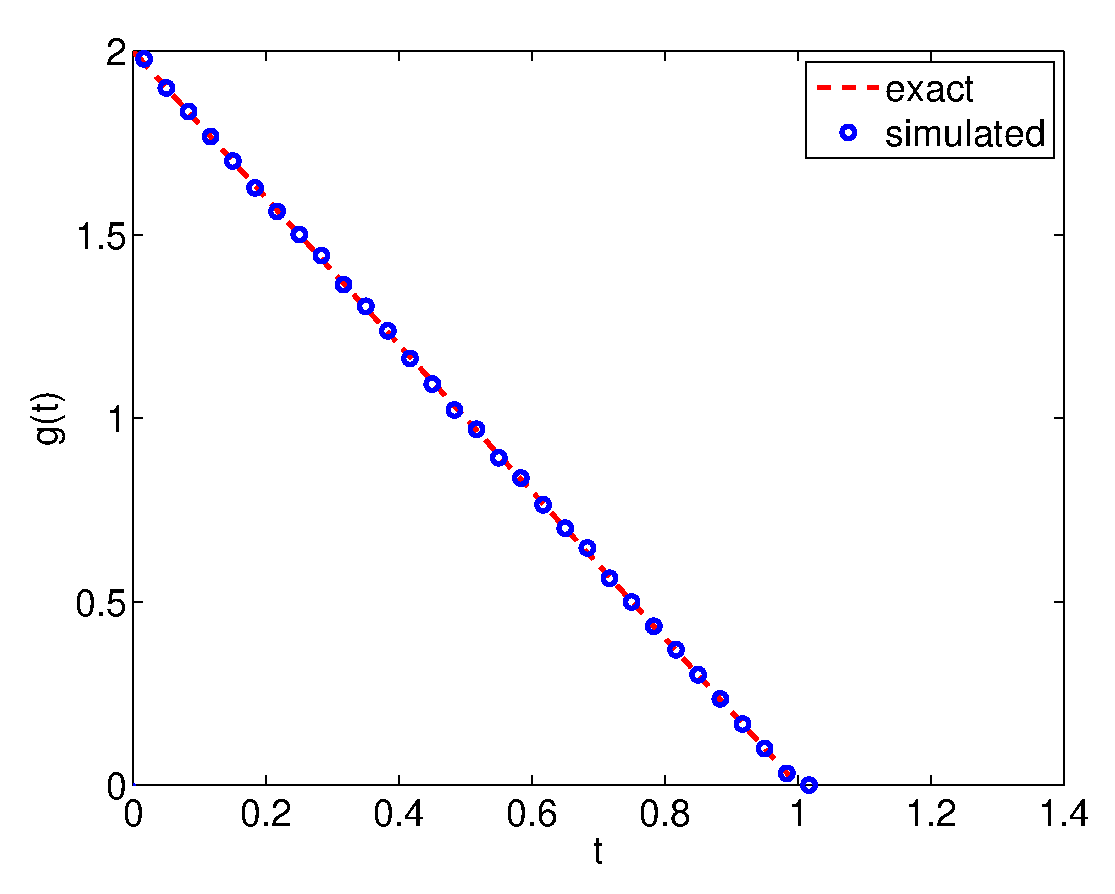
\includegraphics[width=0.48\columnwidth]{../Matlab/Plots/LinePicking_test_sim_line.eps}}
%     \caption{The line-line picking problem ($L=1$).}
%   \end{center} 
% \vspace{-4mm}
% \end{figure}

\subsubsection{PDF}

The elegant feature of this problem is that the Manhattan distance is
made up from the horizontal distance, and the vertical distance, and
these two are independent. Hence the total distance is the sum of two
independent random variables, i.e.,
\[ t_{\rm Manhattan} = t_X + t_Y, \]
where $t_X$ and $t_Y$ are distances given by the line-line picking
problem (Section~\ref{sec:line_line}).


The probability density function of distances between two (uniformly)
randomly chosen points on the unit line is given in
\eqref{eq:line_lineL}, and so the densities in the $X$ and $Y$
directions for a rectangle with sides $a$ and $b$ will be
\begin{eqnarray}
  \label{eq:rect_xy}
  g^{\rm X}_b(t) & = & \left\{ \begin{array}{ll}
                    \frac{2}{b} \left( 1-\frac{t}{b} \right), &
                         \mbox{ for } 0 \leq t \leq b, \\
                    0, & \mbox{ otherwise}, \\
                  \end{array} \right. \nonumber \\
  g^{\rm Y}_a(t) & = & \left\{ \begin{array}{ll}
                    \frac{2}{a} \left( 1-\frac{t}{a} \right), &
                         \mbox{ for } 0 \leq t \leq a, \\
                    0, & \mbox{ otherwise}. \\
                  \end{array} \right. \nonumber 
\end{eqnarray}
The density for the Manhattan distance will be the convolution of
these, i.e., for $0 \leq t \leq a+b$, and $a \leq b$, we get
\begin{eqnarray}
    g^{\rm X+Y}_b(t) & = & g^{\rm X+Y}_b(t), \nonumber \\
       & = & \left[ g^{\rm Y}_a *  g^{\rm X}_b \right] (t) \nonumber \\
       & = & \int_{-\infty}^{\infty} g^{\rm Y}_a(s)  \, g^{\rm X}_b(t-s) \, ds,  \nonumber \\
       & = & \int_{\max(0,t-b)}^{\min(a,t)} g^{\rm Y}_a(s)  \, g^{\rm X}_b(t-s) \, ds,  \nonumber \\
       & = & \frac{4}{a b} \int_{\max(0,t-b)}^{\min(a,t)}  
              \left( 1-\frac{s}{a} \right) 
              \left( 1-\frac{t-s}{b} \right)  \, ds,  \nonumber \\
       & = & \frac{4}{a b} \int_{\max(0,t-b)}^{\min(a,t)} 
                   \left( 1 - \frac{t}{b} \right)  
                    + \left( \frac{1}{b} - \frac{1}{a} + \frac{t}{a b} \right)  s  
                    - \frac{1}{a b}  s^2 
                \, ds,  \nonumber \\
       & = & \frac{4}{a b} \left[ \left( 1 - \frac{t}{b} \right) s
              + \frac{1}{2} \left( \frac{1}{b} - \frac{1}{a} + \frac{t}{a b} \right)  s^2 
              - \frac{1}{3} \frac{1}{a b}  s^3
                  \right]_{\max(0,t-b)}^{\min(a,t)},  \nonumber \\
       & = & \left\{ \begin{array}{ll}
           \displaystyle
           \frac{4}{a b} \left( 1 - \frac{t}{b} \right) t
              + \frac{2}{a b} \left( \frac{1}{b} - \frac{1}{a} + \frac{t}{a b} \right)  t^2 
              - \frac{4}{3} \frac{1}{a^2 b^2}  t^3, & \mbox{ for } 0 \leq t \leq a, \\
           \displaystyle
           \frac{4}{a b}  \left( 1 - \frac{t}{b} \right) a
              + \frac{2}{a b} \left( \frac{1}{b} - \frac{1}{a} + \frac{t}{a b} \right)  a^2 
              - \frac{4}{3} \frac{1}{a^2 b^2}  a^3, & \mbox{ for } a \leq t \leq b, \\
           \displaystyle
             \frac{4}{a^2 b^2} \int_{0}^{a+b-t} 
                    u(a+b-t - u) \, du
                , & \mbox{ for } b \leq t \leq a + b , \\
                \end{array} \right. \nonumber \\
       & = & \left\{ \begin{array}{ll}
           \displaystyle
           \left(\frac{4}{a b}\right) t
              - \left(\frac{2(a+b)}{a^2 b^2} \right) t^2
              + \left(\frac{2}{3} \frac{1}{a^2 b^2}\right)  t^3, & \mbox{ for } 0 \leq t \leq a, \\
           \displaystyle
                   \left( \frac{6b + 2a}{3b^2} \right)
              - \left( \frac{2}{b^2}  \right) t, & \mbox{ for } a \leq t \leq b, \\
           \displaystyle
              \frac{2(a+b-t)^3}{3 a^2 b^2}
                     , & \mbox{ for } b \leq t \leq a + b,  \\
           \displaystyle
             0, & \mbox{ otherwise}.
                \end{array} \right. \nonumber \\
  \label{eq:manhattan}
\end{eqnarray}
Rearranged:
\begin{equation}
 g^{\rm X+Y}_b(t) =
 \begin{cases}
 \frac{2 t \left(6 a b-3 a t-3 b t+t^2\right)}{3 a^2 b^2}& 0 \le t < a \\
\frac{2 (a+3 b-3 t)}{3 b^2} & a \le t <  b \\
\frac{2 (a+b-t)^3}{3 a^2 b^2} & b \le t \le  a + b\\
 0 & \mbox{otherwise}
 \end{cases}
\end{equation}

\subsubsection{CDF}

The function above is comprised of several polynomial segments. A
closed form for the CDF is therefore easily derived (say by use of
Mathematica), but tiresome and not very instructive ...

Not so tiresome.., took less than typing in the paragraph above!!!
Especially if you use the method i did to get the PDF.

\begin{equation}
 G^{\rm X+Y}_b(t) =
 \begin{cases}
 0 & t < 0\\
\frac{t^2 \left(-4 t (a+b)+12 a b+t^2\right)}{6 a^2 b^2} & 0 \le t < a \\
-\frac{a^2+4 a (b-t)+6 t (t-2 b)}{6 b^2} & a\le t <  b \\
-\frac{a^4+4 a^3 (b-t)+6 a^2 t (t-2 b)+4 a (b-t)^3+(b-t)^4}{6 a^2 b^2} & b \le t < \le  a + b\\
 1 & t > a + b
 \end{cases}
\end{equation}


\subsubsection{Moments}

As the $X$ and $Y$ distances are independent, we can form the mean and
variance as the sums of the means and variances of the lin-line
picking problem, i.e.,
\begin{eqnarray}
  \mu^{\rm X+Y} & = & \frac{a+b}{3}, \\
  \label{eq:rect_man_mean}
  \sigma^2_{\rm X+Y}
      & = & \frac{a^{2} + b^2}{18}.
  \label{eq:rect_man_var}
\end{eqnarray}



We can also easily get 

\begin{eqnarray}
 \mu & = \frac{a+b}{3} \\
 \sigma^{2} & = \frac{2 a^5+14 a^4 (b-1)-28 a^3 (b-2) b+35 a^2 b^2 (4 b-1)+105 b^4}{1890 b^2}
\end{eqnarray}






